\section{Phân tích \& Thiết kế hệ thống}
\subsection{Entity Relationship Diagram (ERD)}
\indent \indent Lược đồ bao gồm các thực thể User, Organizer, Event, TicketClass, Purchase, Ticket, ChatSession, Message, Voucher. 
\begin{figure}[H]
    \centering
    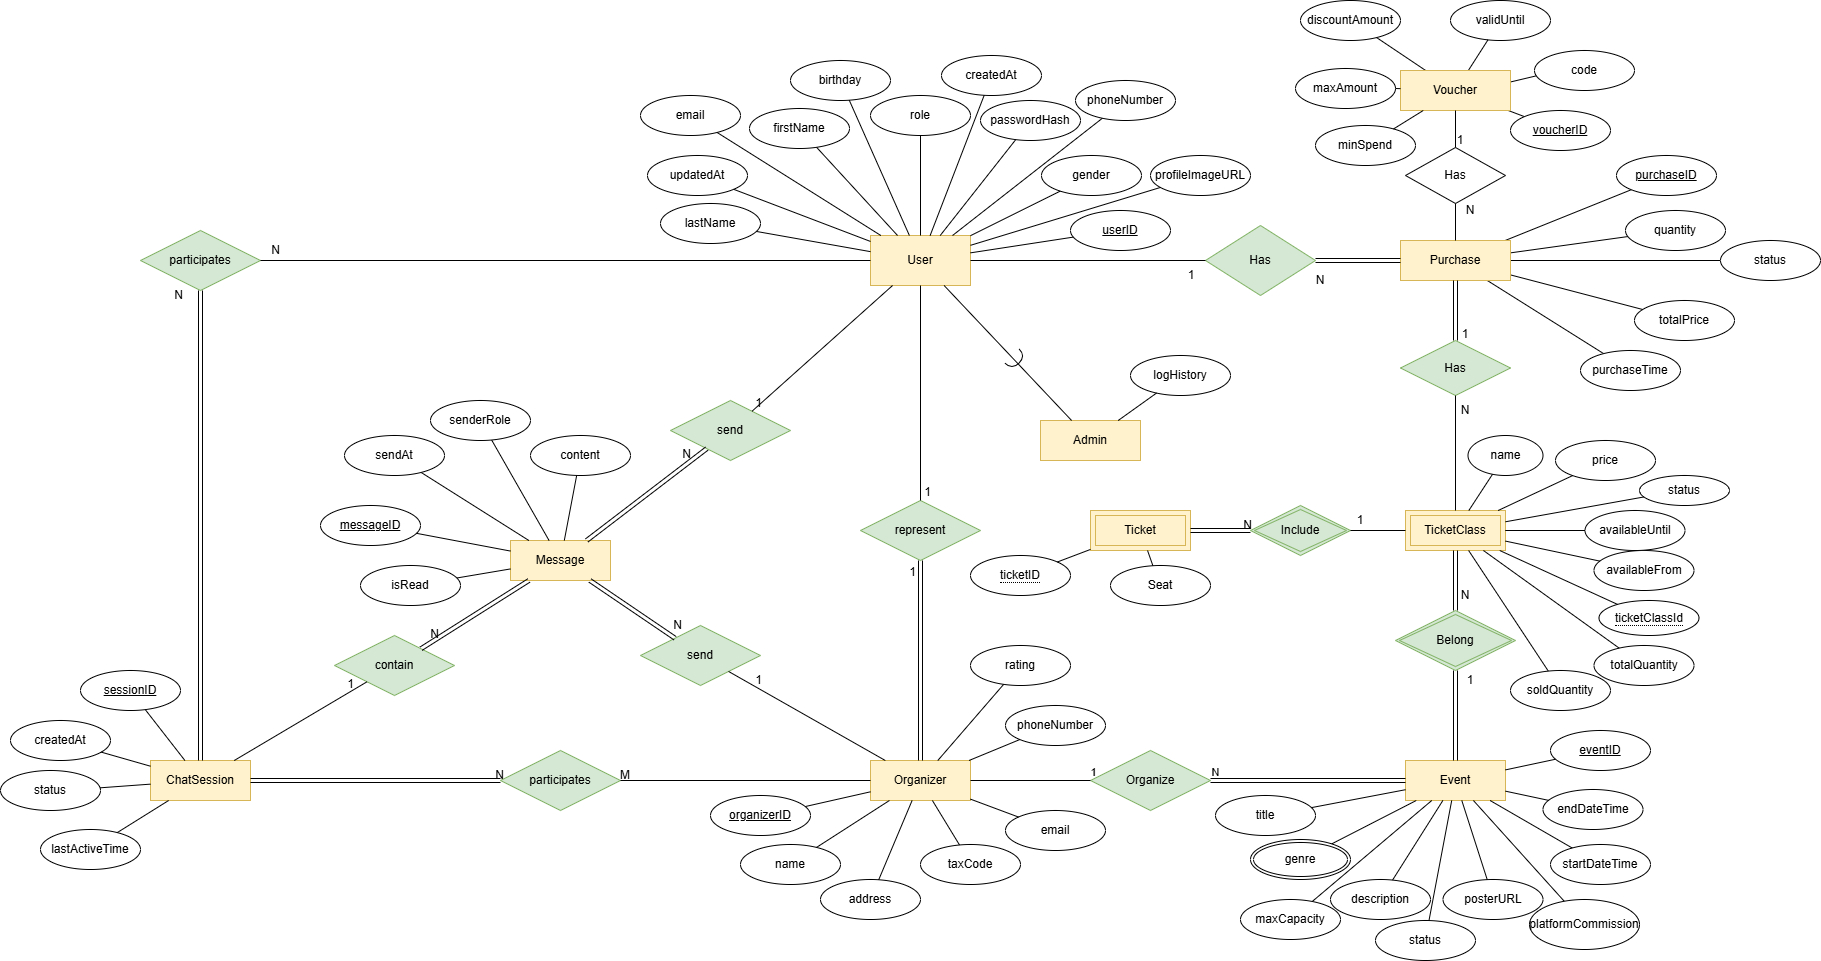
\includegraphics[width=1\textwidth]{Images/ERD.drawio.png}
    \vspace{10pt}
    \caption{Sơ đồ Quan hệ Thực thể (ERD)}
    \label{fig:erd}\end{figure}
\indent Các thực thể này gồm có các thuộc tính:
%==================== USER TABLE ====================
\begin{table}[H]
\centering
\begin{tabular}{|p{4.5cm}|p{6cm}|}
\hline
\textbf{Field} & \textbf{Description} \\ \hline
user\_id (PK) & Primary Key \\ \hline
first\_name & User's first name \\ \hline
last\_name & User's last name \\ \hline
email & Email address \\ \hline
password\_hash & Hashed password \\ \hline
phone\_number & Phone number \\ \hline
gender & Gender \\ \hline
birthdate & Date of birth \\ \hline
profile\_image\_url & Profile image link \\ \hline
role & User role (customer/admin) \\ \hline
created\_at & Account creation time \\ \hline
updated\_at & Last updated time \\ \hline
\end{tabular}
\vspace{15pt}
\caption{Các thuộc tính của thực thể User}
\end{table}

%==================== ORGANIZER TABLE ====================
\begin{table}[H]
\centering
\begin{tabular}{|p{4.5cm}|p{6cm}|}
\hline
\textbf{Field} & \textbf{Description} \\ \hline
organizer\_id (PK) & Primary Key \\ \hline
user\_id & Linked user account \\ \hline
company\_name & Organizer company name \\ \hline
contact\_email & Contact email \\ \hline
contact\_phone & Contact phone number \\ \hline
address & Company address \\ \hline
tax\_code & Tax code \\ \hline
verified\_at & Verification timestamp \\ \hline
\end{tabular}
\vspace{15pt}
\caption{Các thuộc tính của thực thể Organizer}
\end{table}

%==================== EVENT TABLE ====================
\begin{table}[H]
\centering
\begin{tabular}{|p{4.5cm}|p{6cm}|}
\hline
\textbf{Field} & \textbf{Description} \\ \hline
event\_id (PK) & Primary Key \\ \hline
organizer\_id & Linked organizer \\ \hline
title & Event title \\ \hline
genre & Event genre \\ \hline
description & Event description \\ \hline
start\_datetime & Start date and time \\ \hline
end\_datetime & End date and time \\ \hline
poster\_url & Event poster image \\ \hline
max\_capacity & Maximum audience \\ \hline
total\_tickets & Total tickets created \\ \hline
sold\_tickets & Tickets sold \\ \hline
platform\_commission & Platform fee \\ \hline
status & Event status \\ \hline
created\_at & Creation timestamp \\ \hline
updated\_at & Last updated timestamp \\ \hline
\end{tabular}
\vspace{15pt}
\caption{Các thuộc tính của thực thể Event}
\end{table}

%==================== TICKETCLASS TABLE ====================
\begin{table}[H]
\centering
\begin{tabular}{|p{4.5cm}|p{6cm}|}
\hline
\textbf{Field} & \textbf{Description} \\ \hline
ticket\_class\_id (PK) & Primary Key \\ \hline
event\_id & Linked event \\ \hline
name & Ticket class name \\ \hline
price & Ticket price \\ \hline
quantity & Number of tickets \\ \hline
available\_from & Sale start date \\ \hline
available\_until & Sale end date \\ \hline
status & Availability status \\ \hline
\end{tabular}
\vspace{15pt}
\caption{Các thuộc tính của thực thể TicketClass}
\end{table}

%==================== PURCHASE TABLE ====================
\begin{table}[H]
\centering
\begin{tabular}{|p{4.5cm}|p{6cm}|}
\hline
\textbf{Field} & \textbf{Description} \\ \hline
purchase\_id (PK) & Primary Key \\ \hline
user\_id & Buyer ID \\ \hline
voucher\_id & Applied voucher \\ \hline
purchase\_time & Time of purchase \\ \hline
total\_price & Final amount paid \\ \hline
status & Payment status \\ \hline
payment\_method & Payment method \\ \hline
created\_at & Created timestamp \\ \hline
\end{tabular}
\vspace{15pt}
\caption{Các thuộc tính của thực thể Purchase}
\end{table}

%==================== TICKET TABLE ====================
\begin{table}[H]
\centering
\begin{tabular}{|p{4.5cm}|p{6cm}|}
\hline
\textbf{Field} & \textbf{Description} \\ \hline
ticket\_id (PK) & Primary Key \\ \hline
purchase\_id & Linked purchase \\ \hline
ticket\_class\_id & Linked ticket class \\ \hline
seat\_number & Assigned seat \\ \hline
ticket\_code & Ticket code \\ \hline
qr\_code\_url & QR code image \\ \hline
status & Ticket status \\ \hline
issued\_at & Time of issue \\ \hline
used\_at & Time of use \\ \hline
transferred\_to & Recipient ID \\ \hline
recipient\_name & Recipient name \\ \hline
recipient\_phone & Recipient phone number \\ \hline
\end{tabular}
\vspace{15pt}
\caption{Các thuộc tính của thực thể Ticket}
\end{table}

%==================== VOUCHER TABLE ====================
\begin{table}[H]
\centering
\begin{tabular}{|p{4.5cm}|p{6cm}|}
\hline
\textbf{Field} & \textbf{Description} \\ \hline
voucher\_id (PK) & Primary Key \\ \hline
code & Voucher code \\ \hline
discount\_type & Percentage or fixed amount \\ \hline
discount\_value & Discount value \\ \hline
min\_spend & Minimum spend required \\ \hline
max\_discount & Max discount value \\ \hline
valid\_from & Start validity date \\ \hline
valid\_until & End validity date \\ \hline
usage\_limit & Total number of uses allowed \\ \hline
used\_count & Number of times used \\ \hline
applicable\_to & Applicable ticket/event types \\ \hline
created\_by & Creator ID \\ \hline
\end{tabular}
\vspace{15pt}
\caption{Các thuộc tính của thực thể Voucher}
\end{table}

%==================== CHATSESSION TABLE ====================
\begin{table}[H]
\centering
\begin{tabular}{|p{4.5cm}|p{6cm}|}
\hline
\textbf{Field} & \textbf{Description} \\ \hline
session\_id (PK) & Primary Key \\ \hline
title & Session title \\ \hline
created\_at & Creation time \\ \hline
last\_active\_time & Last active timestamp \\ \hline
status & Session status \\ \hline
created\_by & Creator ID \\ \hline
\end{tabular}
\vspace{15pt}
\caption{Các thuộc tính của thực thể ChatSession}
\end{table}

%==================== MESSAGE TABLE ====================
\begin{table}[H]
\centering
\begin{tabular}{|p{4.5cm}|p{6cm}|}
\hline
\textbf{Field} & \textbf{Description} \\ \hline
message\_id (PK) & Primary Key \\ \hline
session\_id & Linked chat session \\ \hline
sender\_id & Sender ID \\ \hline
sender\_role & Sender role (user/admin) \\ \hline
content & Message content \\ \hline
sent\_at & Time sent \\ \hline
is\_read & Read status \\ \hline
read\_at & Time read \\ \hline
\end{tabular}
\vspace{15pt}
\caption{Các thuộc tính của thực thể Message}
\end{table}
\subsection{Kiến trúc hệ thống}
\indent \indent Kiến trúc hệ thống này tuân theo mô hình 3 tầng (Three-tier Architecture), giúp phân tách rõ ràng giữa giao diện người dùng, xử lý nghiệp vụ và lưu trữ dữ liệu. Mô hình này đảm bảo hiệu suất, bảo mật và khả năng mở rộng cao.
\begin{figure}[H]
    \centering
    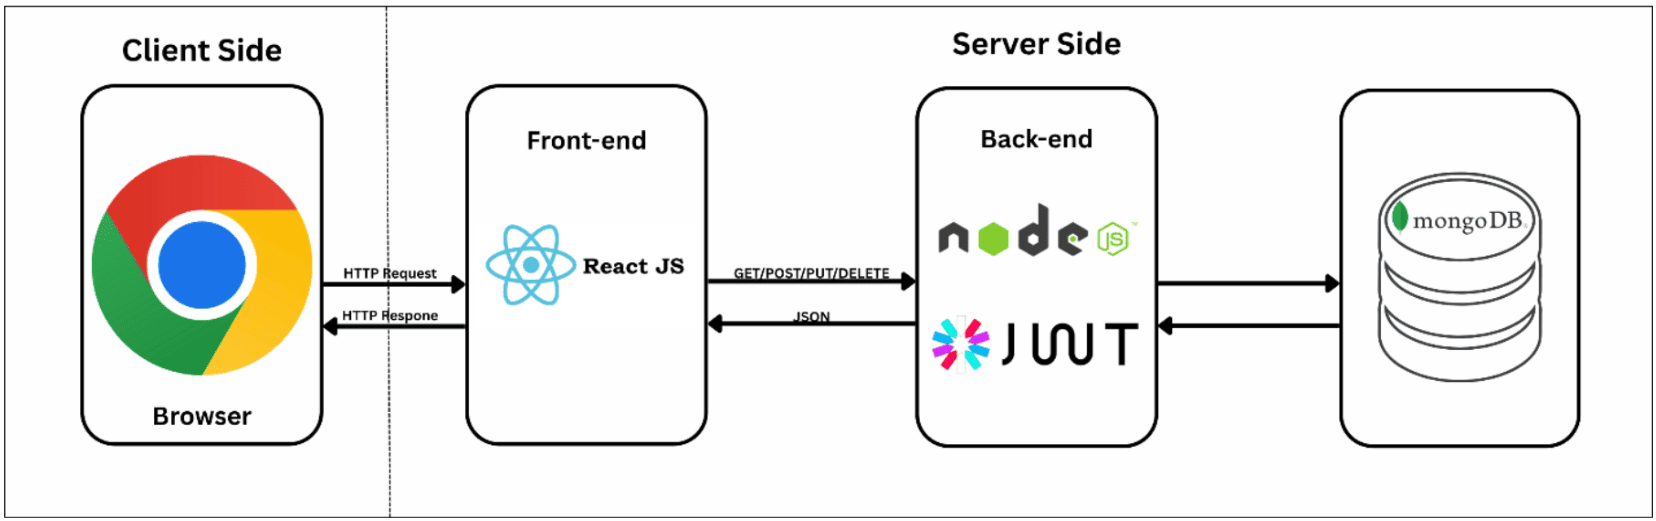
\includegraphics[width=0.8\textwidth]{Images/KienTrucHeThong.png}
    \vspace{10pt}
    \caption{Kiến trúc hệ thống}
    \label{fig:hdfs_architecture}
\end{figure}
\begin{itemize}
    \item[1.] \textbf{Client Side (Trình duyệt \& Giao diện người dùng)}
    \begin{itemize}
        \item[-] Người dùng tương tác với hệ thống thông qua trình duyệt web (ví dụ: Chrome).
        \item[-] Giao diện được xây dựng bằng ReactJS, đảm nhiệm việc hiển thị dữ liệu, nhận yêu cầu và phản hồi từ người dùng.
        \item[-] Giao tiếp với máy chủ thông qua các HTTP Request/Response, sử dụng định dạng JSON để truyền dữ liệu.
    \end{itemize}
    \item[2.] \textbf{Server Side (Back-end \& Xử lý nghiệp vụ)}
    \begin{itemize}
        \item[-] Được phát triển bằng Node.js, đảm nhận xử lý logic nghiệp vụ và điều phối dữ liệu.
        \item[-] Hỗ trợ các phương thức HTTP như GET, POST, PUT, DELETE để thực hiện các thao tác CRUD.
        \item[-] Sử dụng JWT (JSON Web Token) để xác thực và phân quyền người dùng, đảm bảo tính bảo mật trong truy cập tài nguyên.
        \item[-] Là tầng trung gian giữa giao diện người dùng và cơ sở dữ liệu, giúp kiểm soát luồng dữ liệu và logic xử lý.
    \end{itemize}
    \item[3.] \textbf{Database Layer (Lưu trữ dữ liệu)}
    \begin{itemize}
        \item[-] Dữ liệu được lưu trữ trong MongoDB, một hệ quản trị cơ sở dữ liệu NoSQL phổ biến.
        \item[-] Tầng này chịu trách nhiệm lưu trữ, truy xuất và quản lý dữ liệu theo yêu cầu từ tầng hệ thống.
        \item[-] Việc truy cập dữ liệu được kiểm soát thông qua tầng hệ thống, giúp đảm bảo tính toàn vẹn và bảo mật.
    \end{itemize}
    \item[4.] \textbf{Ưu điểm của kiến trúc này}
    \begin{itemize}
        \item[-] Bảo mật cao: Người dùng không truy cập trực tiếp vào cơ sở dữ liệu.
        \item[-] Dễ mở rộng: Có thể triển khai nhiều máy chủ hệ thống để xử lý song song.
        \item[-] Tái sử dụng tốt: Các tầng được tách biệt, dễ bảo trì và nâng cấp.
        \item[-] Hiệu suất ổn định: Phân chia rõ ràng vai trò giữa các tầng giúp tối ưu hóa xử lý.
    \end{itemize}
\end{itemize}
\subsection{Xây dựng mô hình gợi ý sự kiện}
\subsubsection{Mục tiêu mô hình}
\indent \indent Mục tiêu của mô hình là xây dựng tiêu chí lọc "Dành cho bạn" giúp gợi ý những sự kiện phù hợp nhất với từng người dùng dựa trên lịch sử tương tác và đặc điểm sở thích. Mô hình được xây dựng dưới dạng \textbf{Learning to Rank}, trong đó thuật toán \textbf{LightGBM Ranker} được sử dụng nhằm tối ưu thứ tự sắp xếp các sự kiện theo mức độ phù hợp.\\
\indent Cách tiếp cận này cho phép hệ thống hiểu rằng \textit{hành vi mua vé} thể hiện mức độ quan tâm cao hơn \textit{click xem chi tiết}, và \textit{không tương tác}, từ đó xếp hạng các sự kiện theo mức độ ưu tiên cá nhân hóa.
\subsubsection{Dữ liệu đầu vào của mô hình}
\indent \indent Mô hình sử dụng dữ liệu từ ba nhóm chính:\\
\indent \textbf{(1) Dữ liệu tương tác người dùng (Interaction Data)}: 
\begin{itemize}
    \item[-] Xem chi tiết sự kiện (click)
    \item[-] Mua vé (purchase)
    \item[-] Không tương tác (negative samples)
\end{itemize}
\indent \indent Dữ liệu được lưu dưới dạng: \textbf{interactions(user\_id, event\_id, click, purchase, timestamp)}\\
\indent Đây là nguồn dữ liệu cốt lõi giúp mô hình học được mức độ quan tâm thực tế.\\
\indent \textbf{(2) Dữ liệu người dùng (User Features)}
\begin{table}[H]
\centering
\begin{tabular}{|p{5cm}|p{5.5cm}|}
\hline
\textbf{Thuộc tính} & \textbf{Mô tả} \\ \hline
Tuổi & Suy ra sở thích theo độ tuổi \\ \hline
Giới tính & Phục vụ phân tích nhóm khách hàng \\ \hline
Thành phố & Gợi ý sự kiện gần thành phố \\ \hline
Thể loại đã từng tham gia & Biểu diễn sở thích \\ \hline
Mức giá trung bình từng mua & Xác định khả năng chi tiêu \\ \hline
\end{tabular}
\vspace{15pt}
\caption{Các thuộc tính trích xuất từ thông tin người dùng (User Features)}
\end{table}
\indent \textbf{(3) Dữ liệu sự kiện (Event Features)}
\begin{table}[H]
\centering
\begin{tabular}{|p{5cm}|p{5.5cm}|}
\hline
\textbf{Thuộc tính} & \textbf{Mô tả} \\ \hline
Loại sự kiện & Âm nhạc, hội thảo, workshop, ... \\ \hline
Địa điểm & Thành phố \\ \hline
Ngày diễn ra & Ưu tiên sự kiện sắp tới \\ \hline
Giá vé & Liên quan đến khả năng chi tiêu \\ \hline
Lượt xem / vé bán & Chỉ số phổ biến \\ \hline
\end{tabular}
\vspace{15pt}
\caption{Dữ liệu sự kiện (Event Features)}
\end{table}

\indent \textbf{(4) Đặc trưng kết hợp User–Event (Cross Features)}
\begin{table}[H]
\centering
\begin{tabular}{|p{5cm}|p{5.5cm}|}
\hline
\textbf{Đặc trưng} & \textbf{Ý nghĩa} \\ \hline
Khoảng cách giữa user và event theo thành phố & Ưu tiên sự kiện gần \\ \hline
Chênh lệch giá vé so với giá đã mua & Chọn event phù hợp mức giá \\ \hline
Mức độ tương đồng thể loại & Xếp hạng theo sở thích nội dung \\ \hline
\end{tabular}
\vspace{15pt}
\caption{Đặc trưng kết hợp User–Event (Cross Features)}
\end{table}

\subsubsection{Gán nhãn sự kiện}
\indent \indent Hành vi được xem là các mức độ quan tâm khác nhau:
\begin{table}[H]
\centering
\begin{tabular}{|p{3.5cm}|p{6cm}|p{1cm}|}
\hline
\textbf{Hành vi} & \textbf{Mức độ ý nghĩa} & \textbf{Label} \\ \hline
Mua vé & Quan tâm cao nhất & 5 \\ \hline
Click xem chi tiết & Có quan tâm & 3 \\ \hline
Không tương tác & Không phù hợp & 0 \\ \hline
\end{tabular}
\vspace{15pt}
\caption{Gán nhãn dữ liệu huấn luyện}
\end{table}
\indent Mục tiêu của mô hình là \textbf{tối ưu thứ tự sự kiện theo mức độ quan tâm (ranking)}. 
\subsubsection{Quá trình huấn luyện mô hình (Training Pipeline)}
\indent \indent Quy trình gồm các bước:
\begin{itemize}
    \item[1.] \textbf{Tiền xử lý và xây dựng dataset:}
    \begin{itemize}
        \item[-] Gộp dữ liệu user, event và interactions thành dạng (user\_id, event\_id, feature\_vector, label)
        \item[-] Bổ sung negative samples cho các event mà người dùng chưa từng tương tác
        \item[-] Xử lý missing values, chuẩn hoá dữ liệu
    \end{itemize}
    \item[2.] \textbf{Nhóm dữ liệu theo user (Grouping):} Mỗi người dùng là một group vì mô hình so sánh thứ tự event trong cùng nhóm.
    \item[3.] \textbf{Tạo quan hệ xếp hạng (Pairwise Ranking):} Mô hình học thứ tự tương đối: purchase $>$ click $>$ no-interaction
    \item[4.] \textbf{Tối ưu hàm mất mát LambdaRank:} LightGBM sinh ra gradient dựa trên độ thay đổi \textbf{NDCG} khi hai items bị đảo thứ tự, từ đó điều chỉnh cây quyết định để ưu tiên sự kiện phù hợp.
    \item[5.] \textbf{Huấn luyện nhiều vòng (Boosting):} Mỗi cây học phần residual còn lại $\rightarrow$ giúp mô hình tập trung vào gợi ý sai.
\end{itemize}
\indent \indent Kết quả thu được là mô hình có khả năng \textbf{dự đoán điểm phù hợp (score)} cho từng sự kiện.
\subsubsection{Quy trình gợi ý khi người dùng truy cập (Inference Pipeline)}
\indent \indent Khi người dùng mở trang “Sự kiện dành cho bạn”, hệ thống thực thi:
\begin{itemize}
    \item[] \textbf{Bước 1. Chọn danh sách ứng viên (Candidate Generation):} Chọn tiêu chí lọc
    \begin{itemize}
        \item[-] Sự kiện sắp diễn ra
        \item[-] Cùng thành phố với người dùng
        \item[-] Cùng thể loại người dùng từng mua
        \item[-] Sự kiện phổ biến
    \end{itemize}
    \underline{Ưu điểm:} Giảm chi phí tính toán, không cần đưa toàn bộ sự kiện vào mô hình
    \item[] \textbf{Bước 2. Xây dựng feature cho từng (user, event):} Dùng pipeline đã tạo lúc huấn luyện, bỏ qua label.
    \item[] \textbf{Bước 3. Chạy mô hình dự đoán score và sắp xếp giảm dần}
\end{itemize}
\subsubsection{Đầu ra mô hình}
\indent \indent Dữ liệu trả về dưới dạng JSON:
\begin{lstlisting}
{
  "user_id": 12,
  "recommendations": [
    { "event_id": 105, "score": 0.9211 },
    { "event_id": 210, "score": 0.7743 },
    { "event_id": 311, "score": 0.3123 }
  ]
}
\end{lstlisting}


\subsubsection{Vòng lặp cải thiện tự động (Feedback Loop)}
\indent \indent hệ thống hoạt động theo chu trình:
\begin{itemize}
    \item[1.] User tương tác
    \item[2.] Lưu vào interactions
    \item[3.] Sinh dữ liệu huấn luyện mới
    \item[4.] Huấn luyện mô hình định kỳ
    \item[5.] Gợi ý chính xác hơn
\end{itemize}
\indent \indent Mỗi lần người dùng click hoặc mua vé, mô hình sẽ học thêm và điều chỉnh sở thích.
\subsubsection{Tổng quát quy trình hoạt động mô hình}
\begin{itemize}
    \item[1.] Thu thập hành vi người dùng
    \item[2.] Xây dựng features (user, event, cross)
    \item[3.] Label hành vi → training dataset
    \item[4.] Huấn luyện LightGBM Ranker (Ranking)
    \item[5.] Sinh danh sách ứng viên
    \item[6.] Dự đoán score
    \item[7.] Sắp xếp \& trả về Top-K sự kiện phù hợp
    \item[8.] Lưu hành vi mới → học lại
\end{itemize}